\documentclass[11pt,a4paper]{article}

\usepackage[margin=2.4cm]{geometry}
\usepackage[T1]{fontenc}
\usepackage{lmodern}
\usepackage{microtype}
\usepackage{booktabs}
\usepackage{enumitem}
\usepackage{needspace}
\usepackage{graphicx}
\usepackage{tabularx}
\usepackage{xcolor}
\usepackage{tikz}
\usetikzlibrary{positioning,arrows.meta,fit,backgrounds,calc}
\usepackage[colorlinks=true,linkcolor=black,urlcolor=violet]{hyperref}

% ─────────────────────────────────────────────────────────────
%  PLACEHOLDERS — change these five lines, nothing else.
% ─────────────────────────────────────────────────────────────
\newcommand{\coursename}{<course / module name>}
\newcommand{\groupname}{<group name>}
\newcommand{\groupmembers}{<member 1> \and <member 2> \and <member 3>}
\newcommand{\instructor}{<instructor>}
\newcommand{\submissiondate}{<date>}

\definecolor{plum}{HTML}{7B3F61}
\definecolor{shell}{HTML}{F3E7EE}
\definecolor{slate}{HTML}{5A6172}
\definecolor{mist}{HTML}{E6E8EE}

\newcommand{\comp}[1]{\textcolor{plum}{\textbf{#1}}}

\title{\vspace{-1.4cm}\textbf{kcal} — Component-Level Design\\
  \large \coursename}
\author{\groupname\\ \small \groupmembers}
\date{\submissiondate}

\begin{document}
\maketitle
\vspace{-0.6cm}

% ─────────────────────────────────────────────────────────────
\section*{Abstract (updated)}

\textbf{kcal} is a visual degree-plan builder for Krea University (SIAS).
A student picks a programme --- single major, double major, major\,+\,minor, or
major\,+\,minor\,+\,concentration --- and kcal lays out a recommended three- or
four-year plan on a year\,$\times$\,trimester grid. Courses are dragged between a
searchable catalogue and the grid; on every change the plan is re-checked against
the university's real rules (credit floors and ceilings, prerequisite ordering,
which trimester and which year a course is actually offered in, the foundation-core
placement rules, and the audit allowance) and every problem is surfaced as a
plain-language hint rather than a silent failure.

The catalogue, the per-programme requirements and the offering data are
\emph{scraped} from the university's own programme pages and term timetables rather
than hand-typed, so the plan reflects what is genuinely on offer. The application
runs entirely in the browser; a student's plan is autosaved locally and never leaves
their machine.

% ─────────────────────────────────────────────────────────────
\section*{1. Software components}

The system splits along one clean seam: an \emph{offline data pipeline} that runs
before the build and produces static JSON, and a \emph{client-side application} that
consumes it. There is no server and no database at runtime.

\vspace{0.15cm}
\renewcommand{\arraystretch}{1.2}
\noindent\textit{\small Build time --- offline, stdlib-only Python}\\[2pt]
\noindent\begin{tabularx}{\textwidth}{@{}l X l@{}}
\toprule
\textbf{Component} & \textbf{Responsibility} & \textbf{Realised as} \\
\midrule
Scraper & Fetches and parses the university's programme pages (structure tabs, graduation-requirement credit tables); caches raw HTML. & \texttt{scrape\_programmes.py} \\
Catalogue generator & Turns seven term timetables (CSV) into the catalogue: credits, terms offered, eligible years, faculty, and the prerequisite graph. & \texttt{generate.py} \\
Requirements builder & Joins the scrape against the catalogue, resolving website course titles to codes; emits per-programme required sets, choice pools and electives. & \texttt{build\_requirements.py} \\
Bundle slimmer & Strips the generated JSON down to the fields the app reads, and splits course descriptions into a lazily fetched chunk. & Vite plug-in \\
\bottomrule
\end{tabularx}

\vspace{0.45cm}
\needspace{6\baselineskip}
\noindent\textit{\small Runtime --- browser, SvelteKit + TypeScript}\\[2pt]
\noindent\begin{tabularx}{\textwidth}{@{}l X l@{}}
\toprule
\textbf{Component} & \textbf{Responsibility} & \textbf{Realised as} \\
\midrule
Data access layer & Typed reads over the generated JSON plus the programme logic: required/choice/elective sets, substitutes, reachability, recommended pathways. & \texttt{data.ts} \\
Plan engine & \emph{The core.} Holds all plan state and derives every consequence of it: placements, credit totals, the rule checks, the hint list. Single source of truth. & \texttt{plan.svelte.ts} \\
Grades module & Grade scale, weighted TGPA/CGPA, and the ``what do I still need'' recovery calculation. & \texttt{grades.ts} \\
Persistence & Autosave of the working plan, named saved plans, prerequisite overrides, and display settings --- all in \texttt{localStorage}. & \texttt{savedPlans}, \texttt{settings} \\
Presentation & The four-column shell and its panels (below), each a pure view over the engine. & Svelte components \\
Admin tools & Separate route for inspecting the catalogue and editing the prerequisite graph; exports edits as JSON. & \texttt{/admin} \\
\bottomrule
\end{tabularx}

\vspace{0.4cm}
\noindent The presentation layer decomposes into six panels:

\begin{itemize}[leftmargin=1.3em,itemsep=2pt]
  \item \comp{Sidebar} --- programme pickers (degree length, structure, major/minor).
  \item \comp{Catalogue} --- search and subject filters over the course list; emits drag sources.
  \item \comp{OverviewGrid} / \comp{TrimesterZoom} --- the year\,$\times$\,trimester board and its single-trimester zoom, drawn at true credit footprint.
  \item \comp{HintsPanel} --- statistics, choice pools, and the live rule hints.
  \item \comp{DetailsPanel} --- metadata for the selected course.
  \item \comp{GradesPanel} --- grade entry and GPA read-out.
\end{itemize}

\clearpage
% ─────────────────────────────────────────────────────────────
\section*{2. Architecture}

\begin{center}
\begin{tikzpicture}[
  font=\small,
  box/.style={draw=slate!70, fill=white, rounded corners=2pt, align=center,
              minimum height=8mm, inner sep=4pt, text width=30mm},
  core/.style={box, fill=shell, draw=plum, thick},
  data/.style={box, fill=mist!60, text width=26mm},
  flow/.style={-{Stealth[length=2mm]}, slate, thick},
  evt/.style={flow, dashed},
  lbl/.style={font=\scriptsize\itshape, text=slate}
]

% ── build time ──────────────────────────────────────────────
\node[data] (web)  at (0, 0)    {krea.edu.in\\programme pages};
\node[data] (csv)  at (0, -2.2) {term timetables\\(CSV)};

\node[box]  (scrape) at (4.4, 0)    {Scraper};
\node[box]  (gen)    at (4.4, -2.2) {Catalogue\\generator};
\node[box]  (req)    at (9.0, -1.1) {Requirements\\builder};

\node[data, text width=42mm] (json) at (4.4, -4.8)
  {generated JSON\\[1pt]\scriptsize courses · requirements\\\scriptsize programme · department};

\draw[flow] (web) -- (scrape);
\draw[flow] (csv) -- (gen);
\draw[flow] (scrape.east) -| (req.north);
\draw[flow] (gen.east)    -| (req.south);
\draw[flow] (gen)  -- (json);
\draw[flow] (req.east) -- ++(0.3,0) |- (json.east);

\begin{scope}[on background layer]
  \node[draw=slate!40, fill=slate!5, rounded corners, inner sep=7pt,
        fit={(web)(csv)(scrape)(gen)(req)(json)(11.1,-1.1)}] (bt) {};
\end{scope}
\node[lbl, anchor=south west] at ([yshift=1pt]bt.north west) {build time (offline)};

% ── runtime ─────────────────────────────────────────────────
\node[box, text width=34mm] (slim) at (4.4, -7.3) {Bundle slimmer\\\scriptsize (Vite plug-in)};
\node[box, text width=40mm] (dal)  at (4.4, -9.1) {Data access layer\\\scriptsize catalogue · programme rules};
\node[core, text width=40mm] (plan) at (4.4, -11.0) {\textbf{Plan engine}\\\scriptsize state · rules · derived hints};
\node[box, text width=24mm] (grades) at (0.1, -11.0) {Grades\\module};
\node[box, text width=24mm] (store)  at (8.7, -11.0) {Persistence\\\scriptsize localStorage};

\draw[flow] (json) -- (slim);
\draw[flow] (slim) -- (dal);
\draw[flow] (dal)  -- (plan);
\draw[flow] (grades) -- (plan);
\draw[{Stealth[length=2mm]}-{Stealth[length=2mm]}, slate, thick] (plan) -- (store);

\node[box, text width=21mm] (cat)   at (0.0, -13.3) {Catalogue};
\node[box, text width=21mm] (side)  at (2.9, -13.3) {Sidebar};
\node[box, text width=21mm] (grid)  at (5.8, -13.3) {Overview\\Grid};
\node[box, text width=21mm] (hints) at (8.7, -13.3) {Hints\\Panel};

\foreach \n in {cat,side,grid,hints}{ \draw[flow] (plan.south) -- (\n.north); }
\draw[evt] ([xshift=4mm]grid.north) -- ([xshift=11mm]plan.south);

\begin{scope}[on background layer]
  \node[draw=plum!40, fill=shell!30, rounded corners, inner sep=7pt,
        fit={(slim)(dal)(plan)(grades)(store)(cat)(hints)}] (rt) {};
\end{scope}
\node[lbl, anchor=south west] at ([yshift=1pt]rt.north west) {runtime (browser)};

\end{tikzpicture}
\end{center}

\noindent Solid arrows carry derived state \emph{down} to the views; the dashed arrow is a
user event calling back \emph{up} into the engine; the double arrow is read/write
persistence. Note that \emph{no} view component talks to another view component ---
every interaction goes through the Plan engine.

% ─────────────────────────────────────────────────────────────
\section*{3. How the components interact}

The architecture is deliberately a \emph{star, not a chain}. One reactive \texttt{Plan}
instance is created by the application shell and passed to every panel as a property.
Panels never hold plan state of their own and never speak to each other:

\begin{enumerate}[leftmargin=1.5em,itemsep=3pt]
  \item \textbf{Views call methods, they do not mutate.} A drag onto the grid calls
    \texttt{plan.place(code, year, trim)}; a programme change calls the picker's setter.
    All writes funnel through the engine.
  \item \textbf{Everything else is derived.} Credit totals, course colours, the filtered
    catalogue, statistics and the hint list are computed \emph{from} plan state, so two
    panels can never disagree --- there is no cache to invalidate.
  \item \textbf{Rules live in exactly one place.} Every check (12-credit floor,
    16/20-credit load, prerequisite order, offering term, year-1 core-only rule, audit
    allowance, total-credit ceiling) is evaluated inside the engine and emitted as a
    typed hint; the HintsPanel merely renders what it is given.
  \item \textbf{Persistence is a side effect, not a step.} An effect watching plan state
    serialises a snapshot to \texttt{localStorage}, keeping a backup of the previous
    value. Restoring re-validates the snapshot before adopting it, so a stale or
    corrupt save can never load a broken plan.
  \item \textbf{The pipeline is upstream and one-way.} The Python components run before
    the build and never at runtime; the application only ever \emph{reads} their output.
    The website remains the source of truth for what a programme requires.
\end{enumerate}

% ─────────────────────────────────────────────────────────────
\section*{4. Sequence: placing a course on the plan}

The interaction below is the system's hot path --- the student drags a course card from
the catalogue onto a trimester slot.

\vspace{0.3cm}
\begin{center}
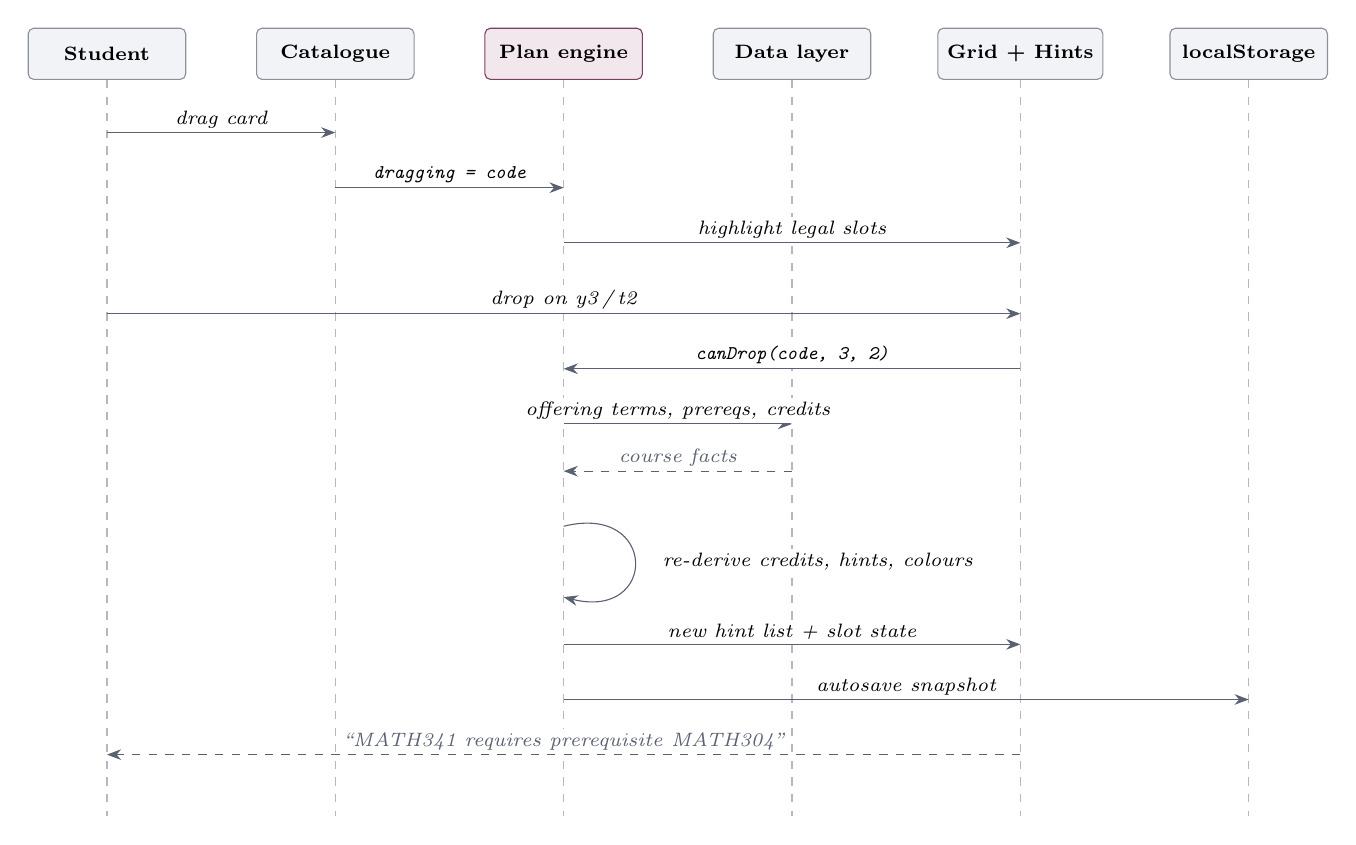
\begin{tikzpicture}[font=\scriptsize,
  actor/.style={draw=slate!70, fill=mist!50, rounded corners=2pt, minimum width=20mm,
                minimum height=6.5mm, align=center, font=\scriptsize\bfseries},
  eng/.style={actor, fill=shell, draw=plum},
  msg/.style={-{Stealth[length=1.8mm]}, slate},
  ret/.style={-{Stealth[length=1.8mm]}, slate, dashed},
  note/.style={font=\scriptsize\itshape, text=slate, fill=white, inner sep=1.5pt}
]

\def\lifelen{9.35}
\foreach \i/\name/\sty in {0/Student/actor, 1/Catalogue/actor, 2/{Plan engine}/eng,
                           3/{Data layer}/actor, 4/{Grid + Hints}/actor, 5/localStorage/actor}{
  \node[\sty] (a\i) at (\i*2.9, 0) {\name};
  \draw[slate!45, dashed] (a\i.south) -- ++(0,-\lifelen);
}

\newcommand{\arrowmsg}[4]{% from, to, y, label
  \draw[msg] (#1*2.9, -#3) -- (#2*2.9, -#3) node[midway, above, note, text=black] {#4};}
\newcommand{\arrowret}[4]{%
  \draw[ret] (#2*2.9, -#3) -- (#1*2.9, -#3) node[midway, above, note] {#4};}

\arrowmsg{0}{1}{1.0}{drag card}
\arrowmsg{1}{2}{1.7}{\texttt{dragging = code}}
\arrowmsg{2}{4}{2.4}{highlight legal slots}
\arrowmsg{0}{4}{3.3}{drop on y3\,/\,t2}
\arrowmsg{4}{2}{4.0}{\texttt{canDrop(code, 3, 2)}}
\arrowmsg{2}{3}{4.7}{offering terms, prereqs, credits}
\arrowret{2}{3}{5.3}{course facts}

\draw[msg] (2*2.9, -6.0) .. controls +(1.2,0.3) and +(1.2,-0.3) .. (2*2.9, -6.9)
  node[midway, right=3mm, note, text=black] {re-derive credits, hints, colours};

\arrowmsg{2}{4}{7.5}{new hint list + slot state}
\arrowmsg{2}{5}{8.2}{autosave snapshot}
\arrowret{0}{4}{8.9}{``MATH341 requires prerequisite MATH304''}

\end{tikzpicture}
\end{center}

\noindent The illegal placement is \emph{not} rejected. The engine accepts the drop and
reports the consequence, because a half-built plan that the student is still working on
is a normal state, not an error --- the hint stays until it is fixed or explicitly waived.

% ─────────────────────────────────────────────────────────────
\section*{5. The components on screen}

\begin{center}
\begin{minipage}{0.92\textwidth}\centering
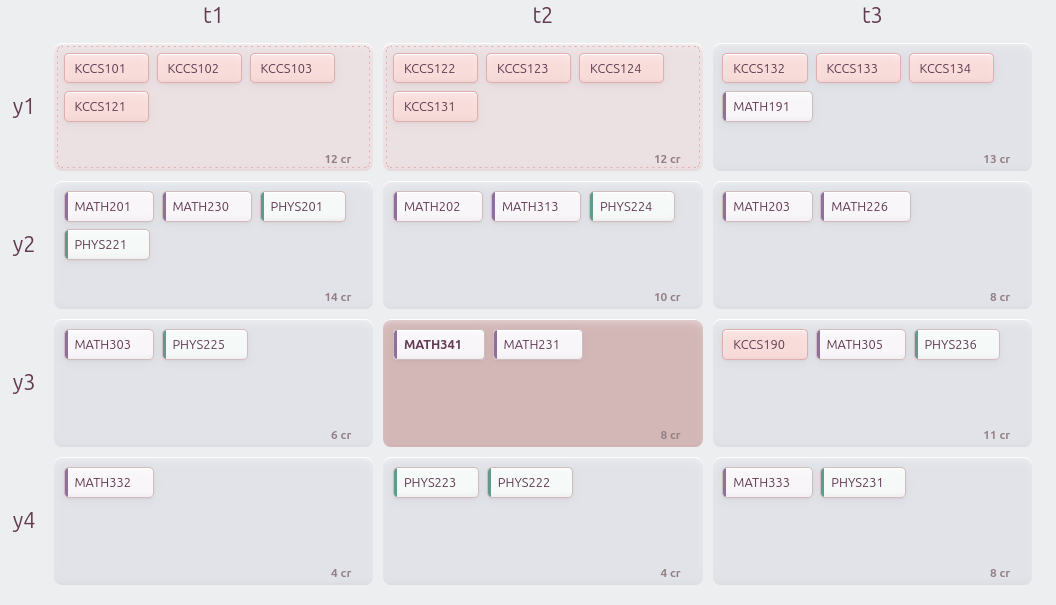
\includegraphics[width=0.93\textwidth]{figs/grid.png}\\[4pt]
{\small \comp{OverviewGrid} --- the year\,$\times$\,trimester board: credit totals per slot,
foundation-core courses in their own colour, year-1 slots marked core-only, and the
offending trimester tinted where a hint applies.}
\end{minipage}
\end{center}

\vspace{0.3cm}
\noindent\begin{minipage}[b]{0.30\textwidth}
\centering

\includegraphics[width=0.92\textwidth]{figs/sidebar.png}\\[3pt]
{\scriptsize \comp{Sidebar}}\\[8pt]

\includegraphics[width=0.92\textwidth]{figs/card.png}\\[3pt]
{\scriptsize \comp{CatalogueCard}}
\end{minipage}
\hfill
\begin{minipage}[b]{0.30\textwidth}
\centering
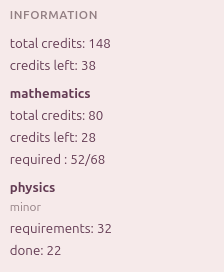
\includegraphics[width=0.78\textwidth]{figs/info.png}\\[3pt]
{\scriptsize \comp{HintsPanel} --- statistics}
\end{minipage}
\hfill
\begin{minipage}[b]{0.32\textwidth}
\centering
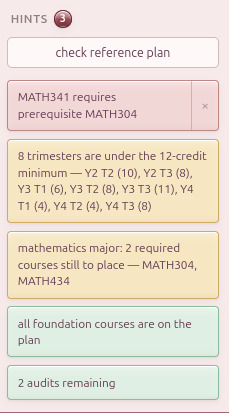
\includegraphics[width=0.80\textwidth]{figs/hints.png}\\[3pt]
{\scriptsize \comp{HintsPanel} --- live hints}
\end{minipage}

\vspace{0.6cm}
\noindent Every number and every hint in the two right-hand panels is derived from the same
\texttt{Plan} instance that draws the grid --- which is why the ``2 required courses still
to place'' count, the prerequisite hint, and the tinted slot on the board can never drift
apart.

\end{document}
